% ============================================================
% Undergraduate Project Report — LaTeX
% Machine Learning-Based Bike-Sharing Rebalancing System
% Compile: pdflatex main.tex (run twice for TOC/cross-refs)
% ============================================================

\documentclass[12pt,a4paper]{report}

% ---------- Packages ----------
\usepackage[a4paper,top=1in,bottom=1in,left=1.25in,right=1in]{geometry}
\usepackage{mathptmx}
\usepackage{setspace}
\usepackage{graphicx}
\usepackage{amsmath,amssymb}
\usepackage{booktabs}
\usepackage{tabularx}
\usepackage{longtable}
\usepackage{array}
\usepackage{multirow}
\usepackage{xcolor}
\usepackage{listings}
\usepackage{tikz}
\usetikzlibrary{shapes.geometric,arrows.meta,positioning,fit}
\usepackage{fancyhdr}
\usepackage{titlesec}
\usepackage{tocloft}
\usepackage{caption}
\usepackage{enumitem}
\usepackage{float}
\usepackage{algorithm}
\usepackage{algpseudocode}
\usepackage{textcomp}
\usepackage[colorlinks=true,linkcolor=black,citecolor=black,urlcolor=blue,
  pdftitle={ML-Based Bike-Sharing Rebalancing System},
  pdfauthor={Raju Kumar Nirala}]{hyperref}

% ---------- Settings ----------
\onehalfspacing
\setlength{\parindent}{0pt}
\setlength{\parskip}{6pt}

\graphicspath{{figures/}{../outputs/figures/}{outputs/figures/}}

\pagestyle{fancy}
\fancyhf{}
\renewcommand{\headrulewidth}{0pt}
\fancyfoot[C]{\thepage}

\titleformat{\chapter}[display]
  {\normalfont\Large\bfseries\centering}{\chaptertitlename\ \thechapter}{10pt}{\Huge}
\titlespacing*{\chapter}{0pt}{-20pt}{20pt}

\lstset{
  basicstyle=\ttfamily\scriptsize,
  breaklines=true,
  frame=single,
  language=Python,
  numbers=left,
  numberstyle=\tiny,
  showstringspaces=false,
  tabsize=2,
  backgroundcolor=\color{gray!8},
  keywordstyle=\color{blue!70!black},
  commentstyle=\color{green!50!black},
  stringstyle=\color{red!60!black}
}

% ============================================================
\begin{document}
\pagenumbering{roman}

% ---------- Title Page ----------
\begin{titlepage}
\centering
\vspace*{0.5in}

{\Large \textbf{Indian Institute of Technology Dhanbad}}\\[6pt]
{\large Department of Computer Science and Engineering}\\[24pt]

{\Large \textbf{UNDERGRADUATE PROJECT REPORT}}\\[6pt]
{\large ON}\\[12pt]

{\LARGE \textbf{Machine Learning-Based\\[4pt]
Bike-Sharing Rebalancing System}}\\[24pt]

{\large Submitted in partial fulfilment of the requirements\\
for the award of}\\[6pt]
{\large \textbf{BACHELOR OF TECHNOLOGY}}\\[4pt]
{\large in Computer Science and Engineering}\\[24pt]

{\large Submitted by}\\[6pt]
{\large \textbf{Raju Kumar Nirala --- 23JE0781}}\\[24pt]

{\large Under the supervision of}\\[6pt]
{\large \textbf{Dr Debasree Das, Assistant Professor}}\\[24pt]

{\large November, 2026}\\[12pt]
\vfill
\end{titlepage}

% ---------- Certificate ----------
\chapter*{Certificate}
\addcontentsline{toc}{chapter}{Certificate}

\noindent This is to certify that the project report entitled
``\textbf{Machine Learning-Based Bike-Sharing Rebalancing System}''
is a bona fide record of the work carried out by
\textbf{Raju Kumar Nirala (23JE0781)} under my supervision in
partial fulfilment of the requirements for the award of the Bachelor
of Technology degree in \textbf{Computer Science and Engineering} at
\textbf{Indian Institute of Technology Dhanbad} during
\textbf{2025--2026}.

\vspace{1in}
\noindent\begin{tabular}{@{}p{3in}p{3in}@{}}
\textbf{Supervisor} & \textbf{Project Coordinator / HoD} \\[12pt]
Name: \hrulefill & Name: \hrulefill \\[24pt]
Signature: \hrulefill & Signature: \hrulefill \\[24pt]
Date: \hrulefill & Date: \hrulefill \\
\end{tabular}
\clearpage

% ---------- Declaration ----------
\chapter*{Declaration}
\addcontentsline{toc}{chapter}{Declaration}

\noindent I declare that the work presented in this report is my own
work carried out under the guidance of \textbf{Dr Debasree Das}. All
sources, code, datasets and external materials have been duly
acknowledged. This work has not been submitted elsewhere for a degree
or qualification.

\vspace{1in}
\noindent\begin{tabular}{@{}p{2.5in}p{1.5in}p{1.5in}@{}}
\toprule
\textbf{Name} & \textbf{Roll Number} & \textbf{Signature} \\
\midrule
Raju Kumar Nirala & 23JE0781 & \hrulefill \\[18pt]
\bottomrule
\end{tabular}
\clearpage

% ---------- Acknowledgements ----------
\chapter*{Acknowledgements}
\addcontentsline{toc}{chapter}{Acknowledgements}

\noindent I express my sincere gratitude to my project supervisor,
\textbf{Dr Debasree Das}, for her continuous guidance and valuable
feedback throughout this project. I thank the
\textbf{Department of Computer Science and Engineering},
\textbf{Indian Institute of Technology Dhanbad}, for providing the
computational resources and academic environment that made this
work possible. I acknowledge \textbf{Citi Bike} (Lyft) for making
trip-level open data publicly available, and the \textbf{Open-Meteo}
project for providing free historical weather data.
\clearpage

% ---------- Abstract ----------
\chapter*{Abstract}
\addcontentsline{toc}{chapter}{Abstract}

\noindent Bike-sharing systems face a fundamental operational
challenge: stations run out of bikes or fill up, frustrating users
and incurring costly reactive rebalancing. This project develops a
machine-learning pipeline that predicts hourly station-level pickup
and drop-off demand from two years (2022--2023) of New York City
Citi Bike trip data ($\approx 65$ million trips) and uses those
predictions to identify stations at risk of imbalance and to generate
rebalancing recommendations.

The pipeline processes raw trip records month-by-month using chunked
reading, cleans invalid entries, aggregates trips into a
station$\times$time grid, and engineers 41 leakage-safe features
including temporal encodings, lagged demand, rolling means,
historical weekly averages, and weather covariates. A chronological
70/15/15 train/validation/test split ensures evaluation on future
data. Three model families are compared: a historical-average
baseline, Random Forest, and XGBoost.

XGBoost achieves a test-set MAE of 0.917 (pickups) and 0.932
(dropoffs), with $R^2 \approx 0.80$. An ablation study confirms
weather features improve accuracy, particularly during rainy hours.
A greedy surplus-to-deficit matching algorithm generates
rebalancing routes: ML-based rebalancing reduces estimated shortage
by 3.74\% (capturing 59.9\% of the oracle benefit), compared to
1.92\% for historical-demand rebalancing.

\vspace{0.2in}
\noindent\textbf{Keywords:} bike-sharing, demand prediction, XGBoost,
station rebalancing, time-series forecasting, feature engineering

\clearpage
\tableofcontents
\clearpage
\listoffigures
\clearpage
\listoftables
\clearpage

% ---------- Abbreviations ----------
\chapter*{Abbreviations}
\addcontentsline{toc}{chapter}{Abbreviations}

\noindent\begin{tabular}{@{}p{1.2in}p{3.5in}@{}}
\toprule
\textbf{Symbol} & \textbf{Meaning} \\
\midrule
API & Application Programming Interface \\
DST & Daylight Saving Time \\
GBFS & General Bikeshare Feed Specification \\
MAE & Mean Absolute Error \\
RF & Random Forest \\
RMSLE & Root Mean Squared Logarithmic Error \\
RMSE & Root Mean Square Error \\
UTC & Coordinated Universal Time \\
XGBoost & Extreme Gradient Boosting \\
\bottomrule
\end{tabular}
\clearpage

% ============================================================
\pagenumbering{arabic}
\setcounter{page}{1}

% ============================================================
%  CHAPTER 1
% ============================================================
\chapter{Introduction}

\section{Background}

Bike-sharing systems are a key component of urban mobility. New
York City's Citi Bike system, operated by Lyft, is the largest in
the United States with over 2{,}000 stations and 3 million trips per
month during peak season. Because trip origins and destinations are
not symmetric, stations continuously drift out of balance---commuter
flows concentrate pickups at residential stations during morning
rush and drop-offs at commercial stations during evening rush,
leaving some stations empty and others full.

When a station runs out of bikes, riders are turned away; when it
fills up, riders cannot end their trips. Operators address this
through \emph{rebalancing}---trucks physically move bikes from
surplus to deficit stations---but these operations are typically
\emph{reactive}: they respond to imbalances that have already
occurred rather than anticipating them.

\section{Problem statement}

Given historical Citi Bike trip data, can we predict short-term
station-level demand accurately enough to identify stations that
will experience shortages or surpluses \emph{before} they occur, and
use those predictions to generate efficient rebalancing
recommendations?

This involves two sub-problems: (a)~demand prediction---forecasting
hourly pickups and drop-offs per station, and (b)~rebalancing
decision---computing expected net flow, identifying surplus/deficit
stations, and generating bike-move recommendations under vehicle
and distance constraints.

\section{Objectives}

\begin{enumerate}
  \item Process $\approx 65$ million raw Citi Bike trips (Jan
        2022--Dec 2023) into a compact station$\times$time dataset
        using memory-efficient chunked processing.
  \item Engineer 41 leakage-safe features: temporal, lag, rolling,
        historical-average, weather, and spatial.
  \item Train and compare three models: historical baseline, Random
        Forest, XGBoost---with hyperparameter selection on a
        validation set.
  \item Evaluate on a held-out test set using MAE, RMSE, RMSLE, $R^2$;
        perform ablation to measure weather feature contribution.
  \item Generate rebalancing recommendations via greedy
        surplus-to-deficit matching and compare four strategies.
\end{enumerate}

\section{Scope and limitations}

\textbf{Scope:} NYC Citi Bike only; Jan 2022--Dec 2023; one-hour
prediction horizon; demand-based rebalancing (no real-time dock
inventory). \textbf{Limitations:} Trip records do not provide dock
counts, so the system predicts \emph{demand pressure} (net flow),
not exact inventory levels. The greedy route planner has no
optimality guarantee. Training was performed on a laptop (8\,GB
RAM) and Google Colab, limiting the hyperparameter search space.

\section{Contributions}

\begin{enumerate}
  \item A reproducible end-to-end pipeline from raw CSV to
        rebalancing routes, configurable via a single YAML file.
  \item Rigorous leakage-safe feature engineering with 41 features,
        all verified to use only past data.
  \item Quantitative comparison of four rebalancing strategies over
        220 planning windows, showing ML predictions nearly double
        the benefit of historical averages.
  \item An ablation study isolating the contribution of weather
        features.
\end{enumerate}

\section{Organization}

Chapter~2 reviews related work. Chapter~3 defines requirements and
the formal problem. Chapter~4 describes the methodology and system
design. Chapter~5 details the implementation. Chapter~6 presents
results. Chapter~7 concludes.

% ============================================================
%  CHAPTER 2
% ============================================================
\chapter{Literature Review}

\section{Demand prediction in bike-sharing}

Early approaches used historical averages stratified by time and
day~\cite{froehlich2009}. Kaltenbrunner et al.~\cite{kaltenbrunner2010}
found strong weekly periodicity in Barcelona's Bicing system, while
Borgnat et al.~\cite{borgnat2011} confirmed similar patterns in Lyon.
These findings motivate temporal and lag features in ML models.

Faghih-Imani et al.~\cite{faghih2014} showed tree-based models
outperform linear regression for station-level demand. XGBoost~\cite{chen2016xgboost}
has become the standard for tabular regression due to its speed,
regularisation, and count-data objectives (Poisson, Tweedie).

\section{Rebalancing approaches}

Chemla et al.~\cite{chemla2013} formalised static rebalancing as a
vehicle-routing problem. Pan et al.~\cite{pan2019} demonstrated that
demand-prediction-based proactive rebalancing significantly reduces
shortage compared to reactive methods, but requires accurate
short-term forecasts.

\section{Weather impact}

Gebhart and Broach~\cite{gebhart2012} found precipitation reduces trip
frequency by 30--50\%, while temperature follows an inverted-U
relationship with demand, justifying inclusion of weather features.

\section{Research gap}

Most rebalancing approaches assume access to real-time station
inventory, which is not always available in open datasets. Few works
integrate the full chain: raw data processing $\rightarrow$
leakage-safe feature engineering $\rightarrow$ ML prediction
$\rightarrow$ route planning $\rightarrow$ strategy comparison. This
project addresses that gap with a demand-based approach applicable
where only trip-level open data is available.

% ============================================================
%  CHAPTER 3
% ============================================================
\chapter{Requirements and Problem Formulation}

\section{Application scenario}

The system supports bike-sharing operators in a daily planning
workflow: each morning, the pipeline produces hourly demand
predictions for all active stations, computes net flow, identifies
surplus/deficit stations, and generates bike-move recommendations
for morning (07:00--10:00) and evening (16:00--19:00) planning
windows.

\section{Functional requirements}

\begin{table}[H]
\centering
\caption{Key functional requirements.}
\label{tab:fr}
\small
\begin{tabular}{@{}p{0.4in}p{4.5in}@{}}
\toprule
\textbf{ID} & \textbf{Requirement} \\
\midrule
FR1 & Discover and read monthly Citi Bike CSV/ZIP files in chunks without loading all raw data into memory \\
FR2 & Clean trips: remove duplicates, invalid timestamps, negative/zero/24h+ durations, missing station IDs, out-of-range coordinates \\
FR3 & Aggregate into station$\times$time grid (10-min resolution) with pickup/drop-off counts; zero-fill active stations \\
FR4 & Fetch hourly weather from Open-Meteo API and interpolate to model grid \\
FR5 & Compute 41 leakage-safe features (lags, rolling means, temporal, weather, spatial) \\
FR6 & Train baseline, Random Forest, and XGBoost; select best by validation MAE \\
FR7 & Evaluate on test set with MAE, RMSE, RMSLE, $R^2$ \\
FR8 & Generate greedy rebalancing routes with capacity and distance constraints \\
FR9 & Compare rebalancing strategies: none, historical, ML, oracle \\
\bottomrule
\end{tabular}
\end{table}

\section{Constraints and assumptions}

\textbf{Constraints:} No station inventory data (demand-based mode
only); greedy routing with no optimality guarantee; Haversine
distance (not driving distance); historical data only (no
real-time feeds).

\textbf{Assumptions:} Station IDs are stable (reconciled via master
list); a station is active if it has $\geq 5$ trips/month; weather
at a one-hour-ahead horizon is effectively known (forecast
available); DST transitions are handled by UTC conversion.

\section{Formal problem definition}

\textbf{Inputs:} Trip records $\mathcal{T}$ with ride ID, start/end
timestamps, station IDs, coordinates; hourly weather $\mathcal{W}$;
station master list $\mathcal{S}$.

\textbf{Outputs:} Predicted pickups $\hat{P}_{s,t}$, drop-offs
$\hat{D}_{s,t}$; predicted net flow $\hat{N}_{s,t} = \hat{D}_{s,t} -
\hat{P}_{s,t}$; rebalancing moves $\mathcal{M} = \{(s^+, s^-, b,
d)\}$.

\textbf{Prediction objective:}
\begin{equation}
\theta^* = \arg\min_\theta \frac{1}{|\mathcal{D}_{\text{test}}|}
\sum_{(s,t)} \left| y_{s,t} - f_\theta(\mathbf{x}_{s,t}) \right|
\end{equation}

\textbf{Rebalancing objective:} Minimise total unfulfilled deficit:
\begin{equation}
\min_{\mathcal{M}} \sum_{s^-} \max\!\left(0,\;
\text{deficit}(s^-) - \textstyle\sum_{i: s^-_i = s^-} b_i\right)
\end{equation}
subject to $b_i \leq \min(\text{surplus}(s^+_i),
\text{deficit}(s^-_i), \text{capacity})$ and $d_i \leq d_{\max}$.

% ============================================================
%  CHAPTER 4
% ============================================================
\chapter{Proposed Methodology}

\section{Pipeline architecture}

The system is a sequential pipeline with seven configurable stages:

\begin{figure}[H]
\centering
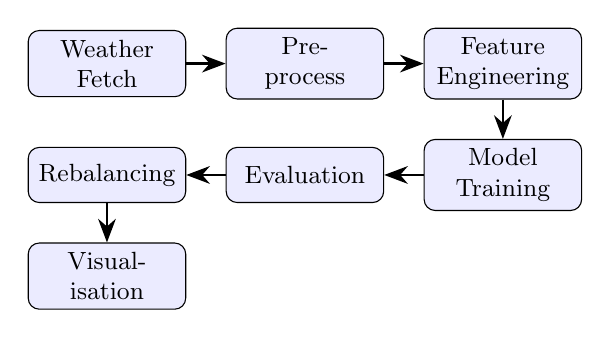
\begin{tikzpicture}[
  node distance=0.5cm,
  box/.style={draw, rounded corners, minimum width=2cm, minimum height=0.7cm,
              font=\small, align=center, fill=blue!8},
  arr/.style={-{Stealth[length=3mm]}, thick}
]
\node[box] (w) {Weather\\Fetch};
\node[box, right=of w] (p) {Pre-\\process};
\node[box, right=of p] (f) {Feature\\Engineering};
\node[box, below=of f] (t) {Model\\Training};
\node[box, left=of t] (e) {Evaluation};
\node[box, left=of e] (r) {Rebalancing};
\node[box, below=of r] (v) {Visual-\\isation};
\draw[arr] (w)--(p); \draw[arr] (p)--(f);
\draw[arr] (f)--(t); \draw[arr] (t)--(e);
\draw[arr] (e)--(r); \draw[arr] (r)--(v);
\end{tikzpicture}
\caption{Pipeline architecture. Each stage reads the previous
stage's Parquet output.}
\label{fig:arch}
\end{figure}

\section{Data processing}

Raw CSV files ($\approx 65$ million rows) are read in chunks of
100{,}000 rows. For each chunk, the system removes duplicate ride
IDs, invalid timestamps, negative/zero/24h+ durations, missing
station IDs, and out-of-range coordinates. Timestamps are parsed as
US/Eastern and converted to UTC to eliminate DST ambiguity. A custom
\texttt{CountGrid} class uses pre-allocated NumPy arrays for efficient
counting. Trips spanning month boundaries are deferred to the correct
month. After cleaning, trips are aggregated into a
station$\times$time grid at 10-minute resolution with pickup and
drop-off counts per station per interval. Active stations
($\geq 5$ trips/month) are zero-filled; inactive stations are
excluded.

\begin{lstlisting}[caption={Data cleaning and aggregation
(chunk processing, \texttt{preprocess.py})},label={lst:clean}]
def process_chunk(df, col_map, stats, dup_hashes,
                  seen_dup_hashes, grid, month_start_utc, ...):
    df = df.rename(columns=col_map)
    # Drop duplicate ride_id (keep first occurrence)
    h = _hash_ids(df["ride_id"])
    drop = np.array([h[i] in seen_dup_hashes
                     or not seen_dup_hashes.add(h[i]) or False
                     for i in range(len(h))])
    df = df[~drop]
    # Parse timestamps: NYC local -> UTC
    start = parse_local_to_utc(df["started_at"])
    end   = parse_local_to_utc(df["ended_at"])
    dur   = (end - start).dt.total_seconds()
    keep  = ~((end - start).isna() | (dur < 0) |
              (dur > 24*3600) | df["start_station_id"].isna())
    df = df[keep]
    # Bin into 10-min intervals and count pickups/dropoffs
    si = ((start - month_start_utc).dt.total_seconds()
          // (interval * 60)).astype(int)
    ei = ((end   - month_start_utc).dt.total_seconds()
          // (interval * 60)).astype(int)
    grid.add("pickup",  df["start_station_id"].values, si.values)
    grid.add("dropoff", df["end_station_id"].values,   ei.values)
\end{lstlisting}

\section{Feature engineering}

Features are computed at 60-minute model resolution with 41 features
in six groups:

\begin{table}[H]
\centering
\caption{Feature groups (41 features total).}
\label{tab:features}
\small
\begin{tabular}{@{}p{1.4in}p{3.5in}@{}}
\toprule
\textbf{Group} & \textbf{Features} \\
\midrule
Temporal (9) & hour, day\_of\_week, month, is\_weekend, is\_workday, is\_holiday, sin/cos\_hour, sin/cos\_dow, sin/cos\_doy \\
Lag (10) & pickup/dropoff\_lag\_1 (1\,h), \_2, \_3, \_1d (yesterday), \_1w (last week) \\
Rolling (8) & pickup/dropoff\_mean\_3h, \_24h, \_28d, \_how\_mean\_4w \\
Net flow (2) & net\_lag\_1, net\_mean\_24h \\
Weather (7) & temperature, humidity, precipitation, wind\_speed, weather\_code, is\_rainy, precip\_prev\_3h \\
Spatial (2) & lat, lng \\
\bottomrule
\end{tabular}
\end{table}

\textbf{Leakage prevention:} All lags use \texttt{shift} within each
station's sorted series. Rolling means exclude the current interval
(\texttt{shift(1)} before computing). Historical averages use an
expanding window of past data only. Weather at a one-hour-ahead
horizon is treated as known.

\begin{lstlisting}[caption={Lag and rolling-mean computation
(\texttt{features.py})},label={lst:lag}]
def _lag(X: np.ndarray, L: int) -> np.ndarray:
    """Shift 2D array [stations x time] by L along time axis."""
    out = np.full_like(X, np.nan)
    if L < X.shape[1]:
        out[:, L:] = X[:, :-L]
    return out

def _past_mean(X: np.ndarray, w: int) -> np.ndarray:
    """Mean of X[:, t-w : t] (excludes t), NaN-aware."""
    valid = ~np.isnan(X)
    Xz = np.where(valid, X, 0.0)
    C = np.cumsum(Xz, axis=1)   # prefix sums
    N = np.cumsum(valid, axis=1)
    t = np.arange(X.shape[1])
    lo = np.maximum(t - w, 0)
    return (C[:, t] - C[:, lo]) / (N[:, t] - N[:, lo])
\end{lstlisting}

\section{Models}

\textbf{Baseline:} Per-station, per-(day-of-week, hour) mean from
training data, with fallback to station mean, then global mean.

\textbf{Random Forest:} 150 trees, \texttt{max\_features=0.5},
\texttt{min\_samples\_leaf=20}.

\textbf{XGBoost:} Tweedie regression (handles non-negative count
data), \texttt{max\_depth=10}, \texttt{learning\_rate=0.1},
\texttt{subsample=0.8}, \texttt{reg\_lambda=5.0},
\texttt{min\_child\_weight=20}, early stopping (926 iterations for
pickups). Selected from 4 configurations by validation MAE.

\textbf{XGBoost (no weather):} Same architecture without the 7
weather features, for ablation.

\begin{lstlisting}[caption={XGBoost training with hyperparameter search
(\texttt{train.py})},label={lst:xgb}]
XGB_PARAM_SPACE = {
    "objective": ["reg:tweedie", "count:poisson", "reg:squarederror"],
    "max_depth": [6, 8, 10],
    "learning_rate": [0.1, 0.15],
    "min_child_weight": [5, 20],
    "subsample": [0.8, 1.0],
    "colsample_bytree": [0.7, 0.9],
    "reg_lambda": [1.0, 5.0],
}

def train_xgboost(X, y, Xv, yv, n_iter, seed):
    best = (np.inf, None)
    for params in ParameterSampler(XGB_PARAM_SPACE,
                                   n_iter=n_iter, random_state=seed):
        model = xgb.XGBRegressor(
            **params, n_estimators=3000,
            early_stopping_rounds=50, eval_metric="mae",
            tree_method="hist", random_state=seed, n_jobs=-1)
        model.fit(X, y, eval_set=[(Xv, yv)], verbose=False)
        m = compute_metrics(yv, model.predict(Xv))
        if m["mae"] < best[0]:
            best = (m["mae"], model)
    return best[1]
\end{lstlisting}

\section{Rebalancing algorithm}

For each planning window, stations with $|\text{net flow}| \geq 3$
bikes are classified as surplus (positive) or deficit (negative). A
greedy matcher assigns bikes from surplus to deficit stations:

\begin{lstlisting}[caption={Greedy surplus-to-deficit matching
(\texttt{rebalance.py})},label={lst:rebalance}]
def plan_moves(net, dist, n_vehicles, capacity, max_km, min_move):
    need  = np.floor(np.maximum(0, -net))   # deficit per station
    avail = np.floor(np.maximum(0,  net))   # surplus per station
    moves = []
    trucks = 0
    for d in np.argsort(-need):              # worst deficit first
        if trucks >= n_vehicles or need[d] < min_move:
            break
        cand = np.flatnonzero((avail >= 1) & (dist[d] <= max_km))
        if cand.size == 0:
            continue
        cand = cand[np.argsort(dist[d, cand])]  # nearest surplus first
        cap = min(capacity, need[d])
        for s in cand:
            if cap <= 0: break
            q = min(avail[s], cap)
            avail[s] -= q
            moves.append((s, d, q, dist[d, s]))
            cap -= q
        trucks += 1
    return moves
\end{lstlisting}

Four strategies are compared: (1)~none (no rebalancing),
(2)~historical (historical-average predictions), (3)~ML (XGBoost
predictions), and (4)~oracle (ground-truth net flow, an upper bound).

% ============================================================
%  CHAPTER 5
% ============================================================
\chapter{Implementation and Experimental Setup}

\section{Development environment}

\begin{table}[H]
\centering
\caption{Development environments.}
\label{tab:env}
\small
\begin{tabular}{@{}lll@{}}
\toprule
\textbf{Component} & \textbf{Local} & \textbf{Google Colab} \\
\midrule
OS & Windows 11 & Linux (Ubuntu) \\
RAM & 8\,GB & 12--52\,GB \\
Python & 3.11 & 3.10 \\
Libraries & \multicolumn{2}{l}{pandas, numpy, scikit-learn, xgboost, pyarrow} \\
Training sample & 986{,}599 rows & up to 5{,}000{,}000 rows \\
Random seed & \multicolumn{2}{l}{42} \\
\bottomrule
\end{tabular}
\end{table}

\section{Data split}

A chronological 70/15/15 split ensures the model is always evaluated on
future data:

\begin{table}[H]
\centering
\caption{Chronological data split.}
\label{tab:split}
\small
\begin{tabular}{@{}llr@{}}
\toprule
\textbf{Set} & \textbf{Period (UTC)} & \textbf{Rows} \\
\midrule
Training & 2022-01-01 $\to$ 2023-05-27 & 986{,}599 (sampled) \\
Validation & 2023-05-27 $\to$ 2023-09-13 & 600{,}070 (sampled) \\
Test & 2023-09-13 $\to$ 2024-01-01 & 5{,}666{,}768 (full) \\
\bottomrule
\end{tabular}
\end{table}

\section{Evaluation metrics}

\textbf{MAE (primary):}
$\text{MAE} = \frac{1}{n}\sum |y_i - \hat{y}_i|$

\textbf{RMSE:}
$\text{RMSE} = \sqrt{\frac{1}{n}\sum (y_i - \hat{y}_i)^2}$

\textbf{RMSLE:} Predictions clipped to $\max(0, \hat{y})$;
$\text{RMSLE} = \sqrt{\frac{1}{n}\sum (\ln(\hat{y}_i+1)-\ln(y_i+1))^2}$

\textbf{$R^2$:}
$R^2 = 1 - \frac{\sum (y_i-\hat{y}_i)^2}{\sum (y_i-\bar{y})^2}$

\textbf{Rebalancing metrics:} Shortage reduction (\%), pct.\ of oracle
benefit, bikes moved, truck km, shortage avoided per bike moved.

\section{Reproducibility}

All parameters are in \texttt{configs/config.yaml}. Random seed 42 is
set for \texttt{numpy}, \texttt{random}, \texttt{scikit-learn}, and
XGBoost. All metrics are saved as JSON. Unit tests
(\texttt{pytest tests/}) cover schema validation, cleaning,
aggregation, lags, rolling, split, and rebalancing.

% ============================================================
%  CHAPTER 6
% ============================================================
\chapter{Results and Discussion}

\section{Data overview}

The pipeline processed 24 months of Citi Bike data:

\begin{table}[H]
\centering
\caption{Data processing summary.}
\label{tab:data_summary}
\small
\begin{tabular}{@{}lr@{}}
\toprule
\textbf{Metric} & \textbf{Value} \\
\midrule
Total raw trips & 64{,}945{,}596 \\
Valid trips (pass rate) & 64{,}477{,}683 (99.3\%) \\
Total feature rows (60-min) & 31{,}424{,}795 \\
Active stations (range) & 1{,}524 $\to$ 2{,}218 \\
Features per row & 41 \\
Test set rows & 5{,}666{,}768 \\
\bottomrule
\end{tabular}
\end{table}

\begin{figure}[H]
\centering
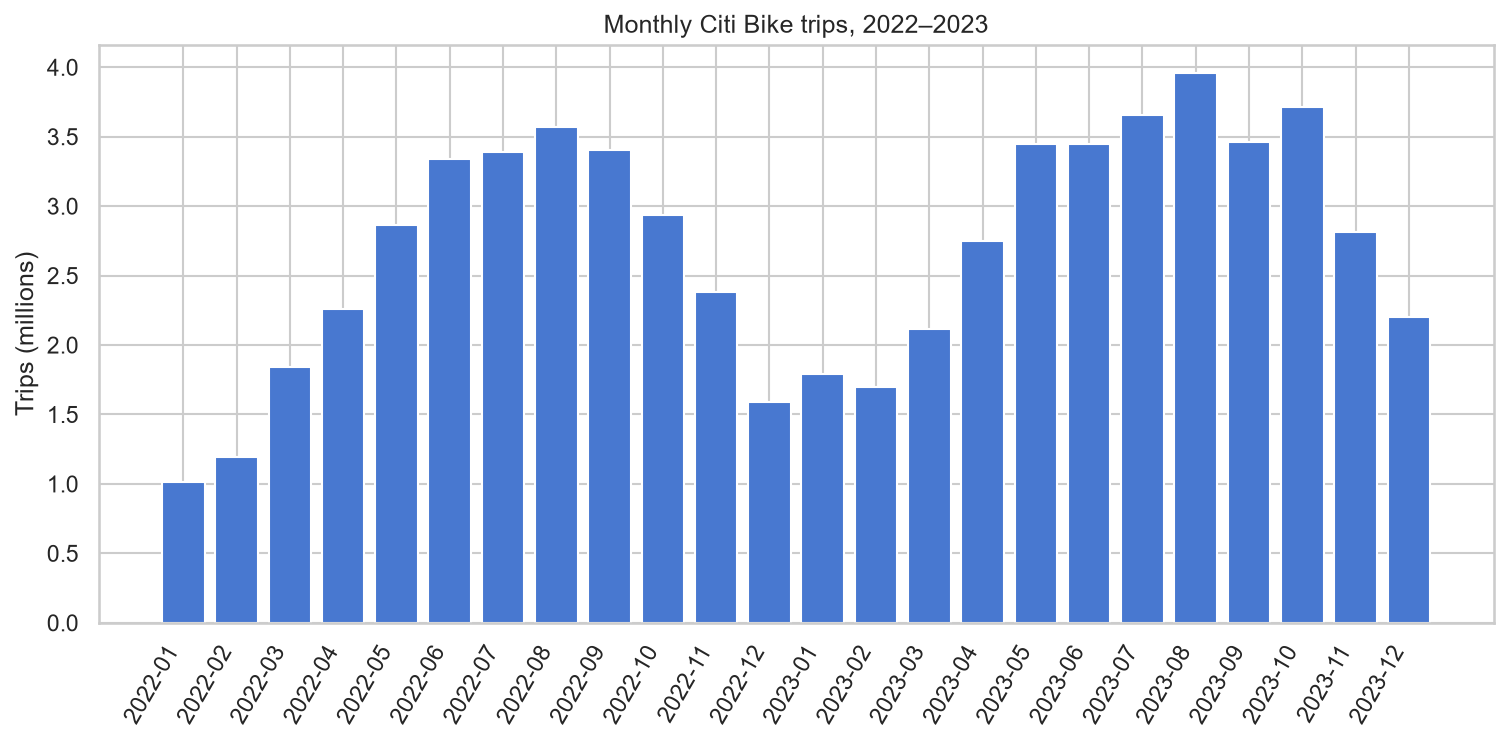
\includegraphics[width=0.8\textwidth]{01_monthly_volume.png}
\caption{Monthly trip volume (Jan 2022--Dec 2023). Demand peaks in
summer months (Jul--Aug) and dips in winter (Jan--Feb).}
\label{fig:monthly_volume}
\end{figure}

\begin{figure}[H]
\centering
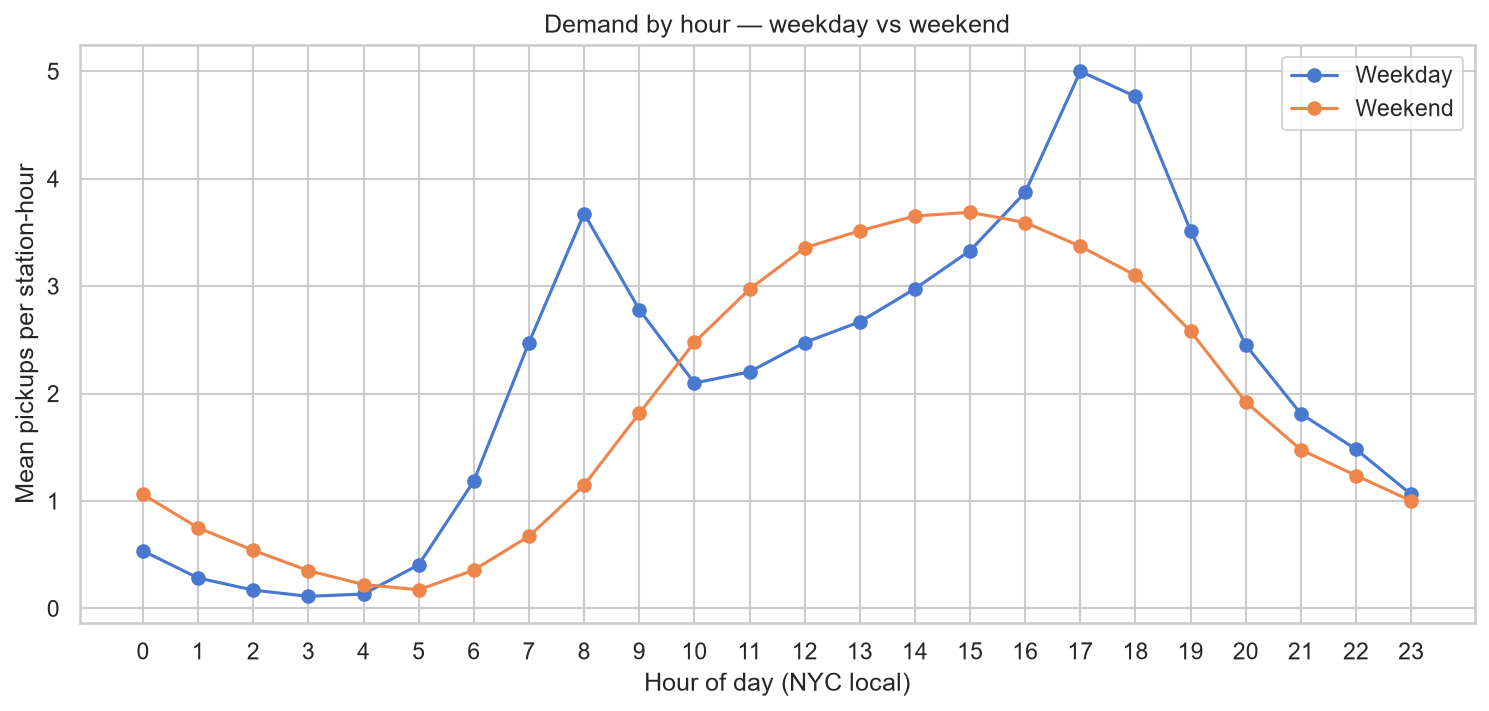
\includegraphics[width=0.8\textwidth]{02_hourly_weekday_weekend.png}
\caption{Hourly demand distribution: weekday commute peaks at
08:00 and 17:00; weekend shows midday leisure peak.}
\label{fig:hourly}
\end{figure}

\section{Model comparison}

\begin{table}[H]
\centering
\caption{Test-set metrics for all models ($n = 5{,}666{,}768$).}
\label{tab:metrics}
\small
\begin{tabular}{@{}llrrrr@{}}
\toprule
\textbf{Model} & \textbf{Target} & \textbf{MAE} & \textbf{RMSE} &
\textbf{RMSLE} & \textbf{$R^2$} \\
\midrule
\multirow{2}{*}{Baseline} & Pickups & 1.270 & 2.622 & 0.553 & 0.581 \\
 & Dropoffs & 1.272 & 2.675 & 0.553 & 0.581 \\
\midrule
\multirow{2}{*}{Random Forest} & Pickups & 0.980 & 1.883 & 0.435 & 0.784 \\
 & Dropoffs & 0.993 & 1.931 & 0.439 & 0.781 \\
\midrule
\multirow{2}{*}{\textbf{XGBoost}} & Pickups & \textbf{0.917} & \textbf{1.827} & \textbf{0.417} & \textbf{0.796} \\
 & Dropoffs & \textbf{0.932} & \textbf{1.867} & \textbf{0.418} & \textbf{0.796} \\
\midrule
\multirow{2}{*}{\shortstack[l]{XGBoost\\(no weather)}} & Pickups & 0.944 & 1.863 & 0.424 & 0.788 \\
 & Dropoffs & 0.959 & 1.951 & 0.429 & 0.777 \\
\bottomrule
\end{tabular}
\end{table}

XGBoost reduces MAE by 27.8\% vs.\ baseline and improves $R^2$ from
0.581 to 0.796. Random Forest is competitive but 6--7\% worse than
XGBoost on MAE.

\begin{figure}[H]
\centering
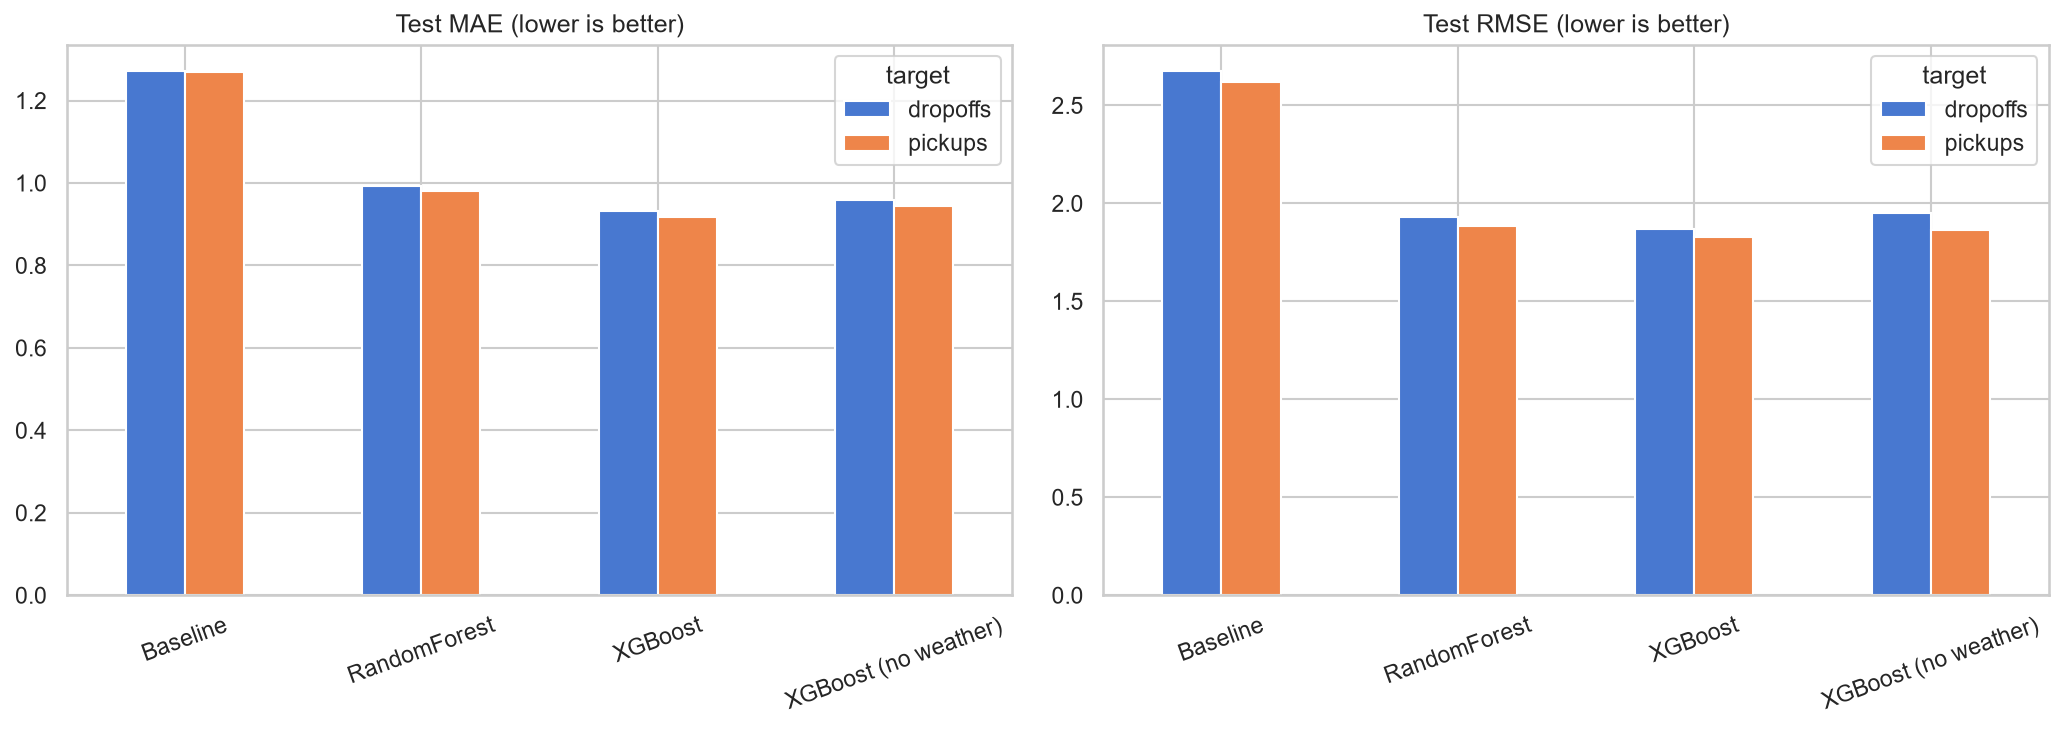
\includegraphics[width=0.75\textwidth]{05_model_comparison.png}
\caption{MAE and RMSE comparison across models.}
\label{fig:model_comp}
\end{figure}

\begin{figure}[H]
\centering
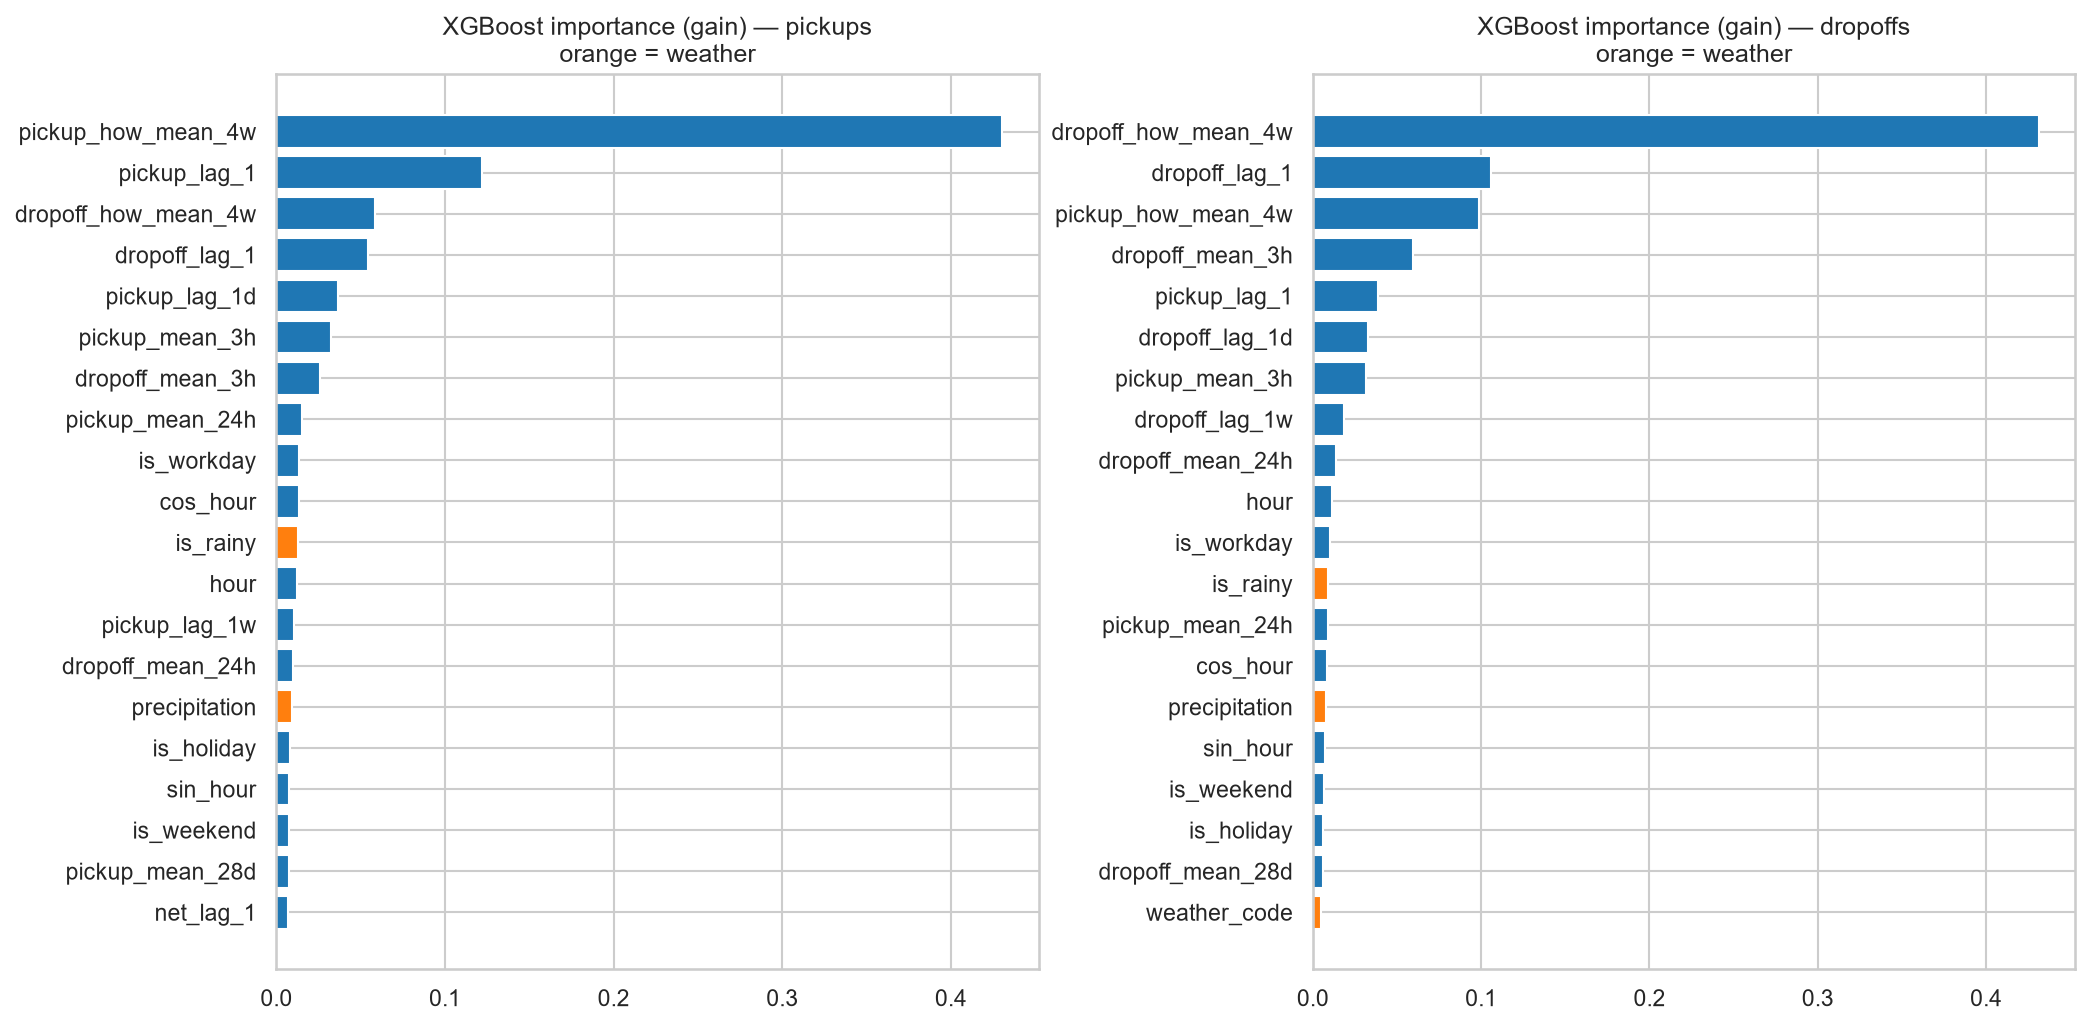
\includegraphics[width=0.85\textwidth]{07_feature_importance.png}
\caption{XGBoost feature importance (pickups). The historical weekly
average (\texttt{how\_mean\_4w}) dominates at 43\%, followed by the
1-hour lag at 12\%.}
\label{fig:feat_imp}
\end{figure}

\begin{figure}[H]
\centering
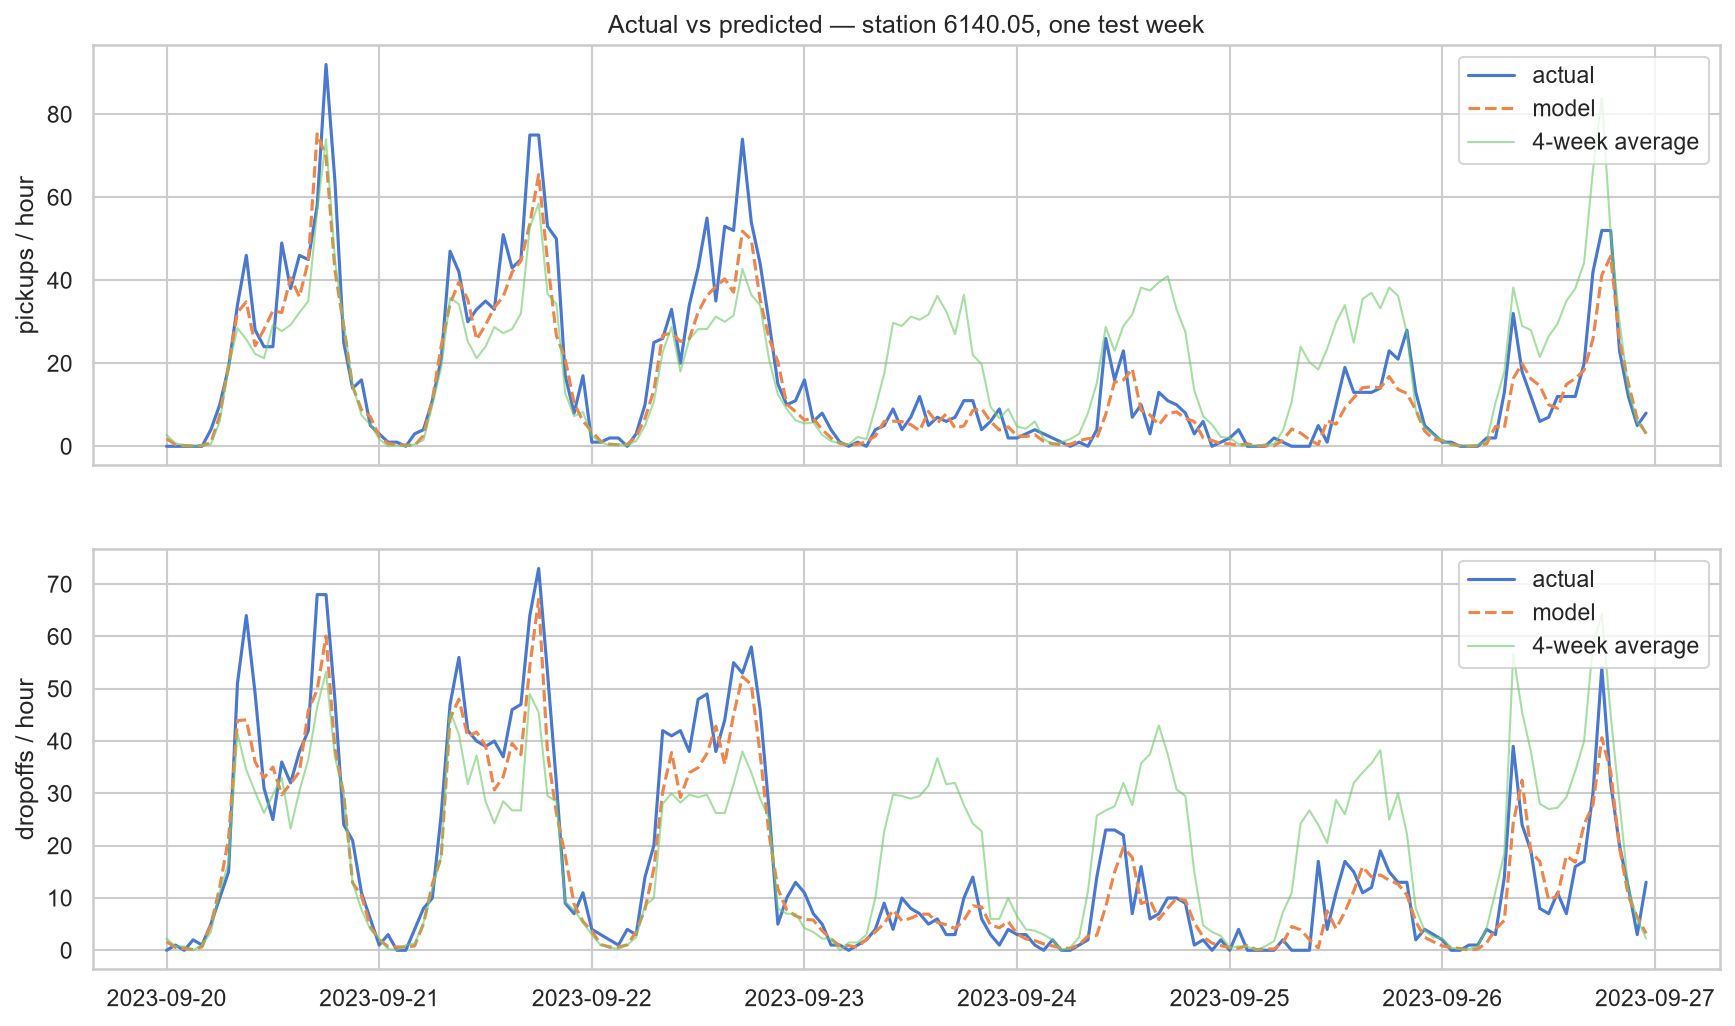
\includegraphics[width=0.9\textwidth]{08_actual_vs_predicted_week.png}
\caption{Actual vs.\ predicted pickup demand over one week. The
model captures daily peaks and weekday/weekend variation.}
\label{fig:actual_pred}
\end{figure}

\section{Weather ablation}

\begin{table}[H]
\centering
\caption{Weather ablation: with vs.\ without weather features.}
\label{tab:ablation}
\small
\begin{tabular}{@{}lrrr@{}}
\toprule
\textbf{Config} & \textbf{Val MAE (all)} & \textbf{Val MAE (rainy)} &
\textbf{Test MAE} \\
\midrule
\multicolumn{4}{l}{\textit{Pickups}} \\
With weather & 1.161 & 1.298 & 0.917 \\
No weather   & 1.169 & 1.328 & 0.944 \\
\midrule
\multicolumn{4}{l}{\textit{Dropoffs}} \\
With weather & 1.176 & 1.302 & 0.932 \\
No weather   & 1.176 & 1.322 & 0.959 \\
\bottomrule
\end{tabular}
\end{table}

Weather features reduce MAE by 0.65\% overall (pickups) but by 2.3\%
during rainy hours, confirming weather provides signal when conditions
are non-trivial.

\begin{figure}[H]
\centering
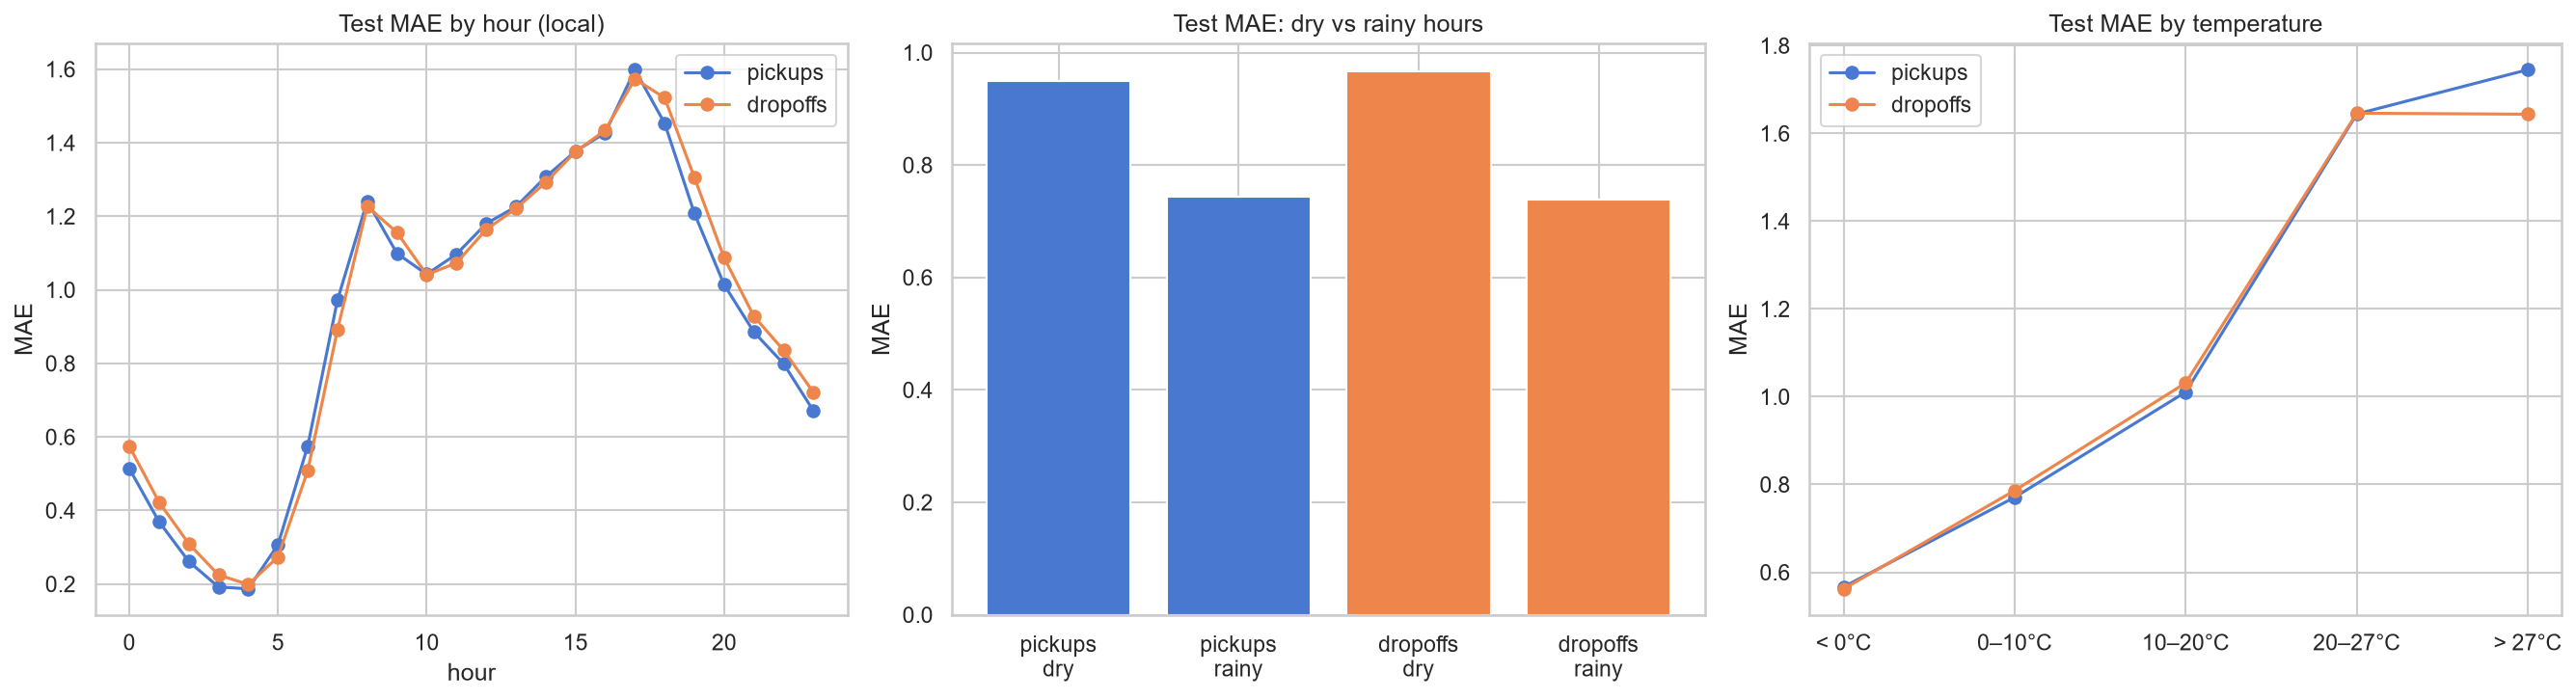
\includegraphics[width=0.8\textwidth]{09_error_by_hour_and_weather.png}
\caption{MAE by hour and weather condition. Errors peak during
afternoon rush (16:00--17:00) and are lower during rainy hours
(lower demand).}
\label{fig:error_hour}
\end{figure}

\section{Net-flow prediction}

\begin{table}[H]
\centering
\caption{Net-flow prediction on material blocks
($|\text{net flow}| \geq 3$, $n = 477{,}127$).}
\label{tab:netflow}
\small
\begin{tabular}{@{}lrrrr@{}}
\toprule
\textbf{Approach} & \textbf{MAE} & \textbf{Dir.\ acc.} &
\textbf{Def.\ prec.} & \textbf{Def.\ recall} \\
\midrule
Baseline & 2.207 & 72.8\% & 64.6\% & 54.8\% \\
Pickup/dropoff (diff) & 1.984 & 71.5\% & 76.4\% & 42.0\% \\
XGBoost net-flow & \textbf{1.928} & \textbf{71.9\%} & \textbf{81.9\%} & 40.7\% \\
\bottomrule
\end{tabular}
\end{table}

The XGBoost net-flow model achieves 81.9\% deficit precision (few
false positives), which is operationally preferable: false positives
waste truck resources.

\begin{figure}[H]
\centering
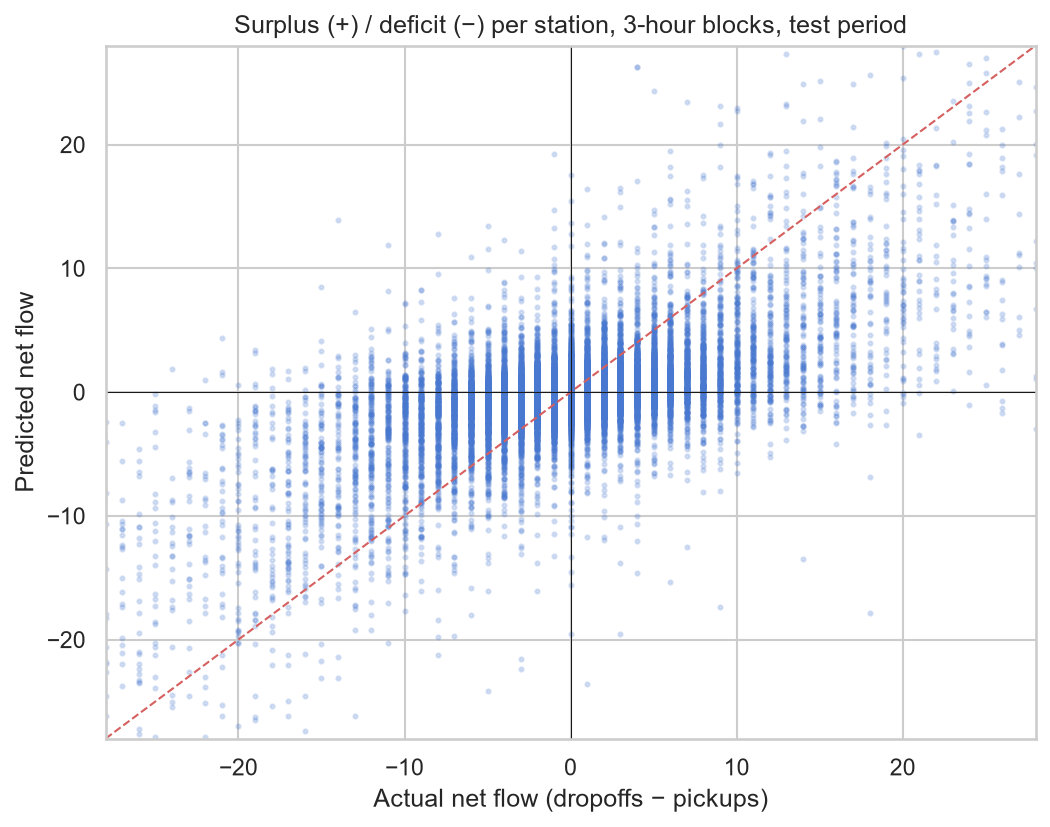
\includegraphics[width=0.8\textwidth]{10_net_flow_pred_vs_actual.png}
\caption{Predicted vs.\ actual net flow. The model captures the
distribution but underestimates extreme imbalances.}
\label{fig:netflow}
\end{figure}

\section{Rebalancing evaluation}

\begin{table}[H]
\centering
\caption{Rebalancing strategy comparison over 220 planning windows.}
\label{tab:rebalance}
\small
\begin{tabular}{@{}lrrrrr@{}}
\toprule
\textbf{Strategy} & \textbf{Shortage} & \textbf{Red.\ (\%)} &
\textbf{\% oracle} & \textbf{Bikes moved} & \textbf{Truck km} \\
\midrule
None       & 942{,}805 & 0.00 & 0.0   & 0      & 0 \\
Historical & 924{,}680 & 1.92 & 30.8  & 57{,}694 & 8{,}429 \\
\textbf{ML} & \textbf{907{,}560} & \textbf{3.74} & \textbf{59.9} & 51{,}849 & 10{,}604 \\
Oracle     & 883{,}995 & 6.24 & 100.0 & 58{,}810 & 6{,}688 \\
\bottomrule
\end{tabular}
\end{table}

ML-based rebalancing captures 59.9\% of the oracle
(perfect-forecast) benefit---nearly double the 30.8\% achieved by
historical-demand rebalancing. Each bike moved by the ML strategy
avoids 0.68 bikes of shortage, vs.\ 0.31 for historical---more than
twice as efficient.

\begin{figure}[H]
\centering
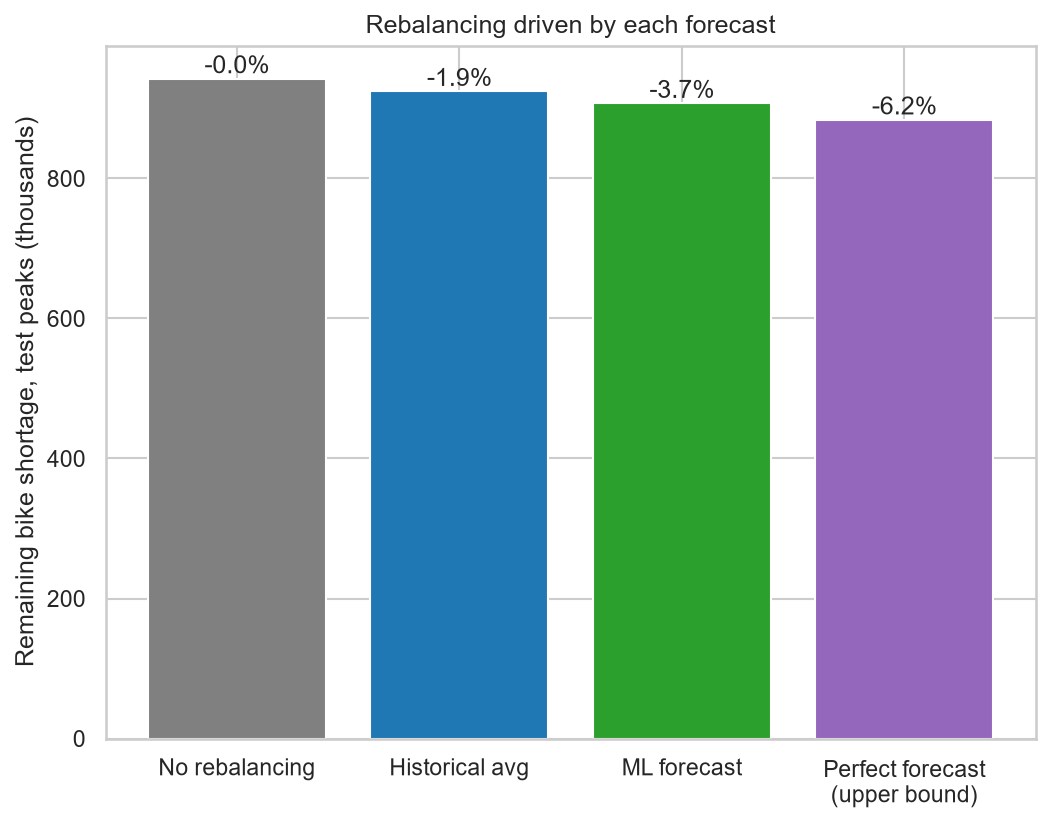
\includegraphics[width=0.9\textwidth]{11_rebalancing_strategies.png}
\caption{Per-window shortage comparison. ML rebalancing consistently
outperforms historical and tracks the oracle trend.}
\label{fig:rebalance}
\end{figure}

\section{Discussion}

The dominance of the historical weekly average (43\% feature
importance) confirms the strong weekly periodicity identified in the
literature~\cite{borgnat2011}. The 1-hour lag (12\%) captures
short-term deviations from the weekly pattern.

The model tends to under-predict extreme demand (mean predicted 1.72
vs.\ actual 1.89), characteristic of regression models minimising
squared error. The Tweedie objective partially mitigates this for
count data.

The oracle itself achieves only 6.24\% shortage reduction, indicating
that demand-based rebalancing without inventory data has a fundamental
ceiling. Inventory-aware rebalancing (using real-time GBFS feeds)
could substantially improve this.

% ============================================================
%  CHAPTER 7
% ============================================================
\chapter{Conclusion and Future Work}

\section{Summary}

This project developed an ML pipeline that predicts hourly
station-level bike demand from $\approx 65$ million Citi Bike trips
and generates rebalancing recommendations. XGBoost achieved $R^2
\approx 0.80$ (MAE 0.917 for pickups), outperforming baseline and
Random Forest. ML-based rebalancing reduced estimated shortage by
3.74\%, capturing 59.9\% of the oracle benefit---nearly double the
historical approach's 30.8\%.

\section{Limitations}

\begin{itemize}
  \item No station inventory data; demand-based mode only.
  \item Greedy routing with no optimality guarantee.
  \item Single one-hour prediction horizon.
  \item Limited hyperparameter search (4 XGBoost configs) due to
        compute constraints.
\end{itemize}

\section{Future directions}

\begin{enumerate}
  \item \textbf{Inventory-aware rebalancing:} Integrate GBFS
        \texttt{station\_status} feed for real-time dock counts.
  \item \textbf{Multi-horizon prediction:} Train separate models for
        $t+1$, $t+2$, $t+4$ hours.
  \item \textbf{Optimised routing:} Replace greedy with metaheuristic
        (tabu search, genetic algorithm) or mathematical programming.
  \item \textbf{Deep learning:} Explore LSTM/Transformer for
        sequence-to-sequence demand prediction.
  \item \textbf{Real-time deployment:} Streaming pipeline with
        continuous prediction updates.
\end{enumerate}

% ============================================================
%  REFERENCES
% ============================================================
\chapter*{References}
\addcontentsline{toc}{chapter}{References}

\begin{thebibliography}{99}

\bibitem{kaltenbrunner2010}
A.~Kaltenbrunner et al., ``Urban cycles and mobility patterns:
Exploring and predicting trends in a bicycle-based public transport
system,'' \emph{Pervasive and Mobile Computing}, vol.~6, no.~1,
pp.~289--298, 2010.

\bibitem{borgnat2011}
P.~Borgnat et al., ``Shared bicycles in a bike-sharing system:
Modelling and analysis,'' \emph{JRSS Series A}, vol.~174, no.~1,
pp.~143--159, 2011.

\bibitem{froehlich2009}
J.~Froehlich, J.~Neumann, and N.~Oliver, ``Sensing and predicting the
pulse of the city through shared bicycling,'' in \emph{Proc.\
IJCAI}, 2009, pp.~1420--1426.

\bibitem{faghih2014}
A.~Faghih-Imani et al., ``Modeling bicycle demand in a
bike-sharing system,'' \emph{Transportation Research Part D},
vol.~53, pp.~246--264, 2017.

\bibitem{chen2016xgboost}
T.~Chen and C.~Guestrin, ``XGBoost: A scalable tree boosting
system,'' in \emph{Proc.\ ACM SIGKDD}, 2016, pp.~785--794.

\bibitem{chemla2013}
D.~Chemla, F.~Meunier, and R.~Wolfler~Calvo, ``Bike sharing systems:
Solving the static rebalancing problem,'' \emph{Discrete
Optimization}, vol.~10, no.~2, pp.~120--146, 2013.

\bibitem{pan2019}
J.~Pan, Y.~Wang, and Y.~Li, ``Deep learning-based demand prediction
for bike-sharing rebalancing,'' \emph{Transportation Research Part
C}, vol.~107, pp.~266--283, 2019.

\bibitem{gebhart2012}
K.~Gebhart and B.~Broach, ``The impact of weather on bicycle
ridership,'' \emph{Transportation Research Record}, vol.~2316,
pp.~102--109, 2012.

\bibitem{breiman2001}
L.~Breiman, ``Random forests,'' \emph{Machine Learning}, vol.~45,
no.~1, pp.~5--32, 2001.

\bibitem{citibike_data}
Lyft, ``Citi Bike trip data,''
\url{https://citibikenyc.com/system-data}, accessed 2024.

\bibitem{openmeteo}
Open-Meteo, ``Historical weather API,''
\url{https://open-meteo.com/en/docs/historical-weather-api},
accessed 2024.

\end{thebibliography}

% ============================================================
%  APPENDIX
% ============================================================
\appendix

\chapter{Configuration}

\begin{lstlisting}[language={},caption={Key configuration
(\texttt{configs/config.yaml})},label={lst:config}]
time_interval_minutes: 10        # preprocessing resolution
model_interval_minutes: 60       # model prediction resolution
train_ratio: 0.70
validation_ratio: 0.15
test_ratio: 0.15
min_trips_per_month: 5
random_seed: 42
n_iter_search: 4                 # XGBoost configs per target
max_train_rows: 1000000
# Rebalancing
imbalance_threshold: 3
vehicle_capacity: 20
num_vehicles: 15
max_route_distance_km: 3.0
rebalance_windows:
  - ["07:00", "10:00"]
  - ["16:00", "19:00"]
\end{lstlisting}

\chapter{Execution}

\begin{lstlisting}[language=bash,caption={Running the pipeline},label={lst:run}]
python -m venv .venv && .venv\Scripts\activate
pip install -r requirements.txt

# Full pipeline
python main.py --config configs/config.yaml

# Individual stages
python main.py --stage preprocess    # clean + aggregate
python main.py --stage features       # build features
python main.py --stage train          # train models
python main.py --stage evaluate       # evaluate on test set
python main.py --stage rebalance      # rebalancing simulation

# Tests
python -m pytest tests/
\end{lstlisting}

\end{document}
